%---------------------------------------------------------------------
% This file provides a skeleton UCL DIS CDT report.
% \pdfinclusioncopyfonts=1
% This command may be needed in order to get \ell in PDF plots to appear. Found in
% https://tex.stackexchange.com/questions/322010/pdflatex-glyph-undefined-symbols-disappear-from-included-pdf
%---------------------------------------------------------------------
% Specify where LaTeX style files can be found.
\newcommand*{\DISCDTLATEXPATH}{latex/}
% Use this variant if the files are in a central location, e.g. $HOME/texmf.
%---------------------------------------------------------------------

\documentclass[NOTE, disdraft=true, UKenglish]{\DISCDTLATEXPATH UCLCDTDISdoc}
% The language of the document must be set: usually UKenglish or USenglish.
% british and american also work!
% Commonly used options:
%  cdtdraft=true|false   This document is an UCL CDT DIS draft.
%  paper=a4|letter       Set paper size to A4 (default) or letter.

%--------------------------------------------------------------------- 
% Add you own definitions here (file dis-gp-defs.sty).
%\usepackage{dis-gp-defs}
%---------------------------------------------------------------------


%--------------------------------------------------------------------- 
% Files with references for use with biblatex.
% Note that biber gives an error if it finds empty bib files.
%\usepackage{biblatex} % uncomment if use addbibresource command
%\addbibresource{dis-gp.bib}
%--------------------------------------------------------------------- 

% Paths for figures - do not forget the / at the end of the directory name.
\graphicspath{{logos/}{figures/}}


%---------------------------------------------------------------------
% Generic document information
%---------------------------------------------------------------------
% Title, abstract and document 
%-------------------------------------------------------------------------
% This file contains the title, author and abstract.
% It also contains all relevant document numbers if needed.
%-------------------------------------------------------------------------

% Partner Logo
% put the name of the logo image file found in graphics path
\DISPartnerLogo{logos/fathom.jpg}


% Title
\DISTitle{Levee Hunter Project Technical Blogpost}

% Draft version:
% If given, adds draft version on front page, a 'DRAFT' box on top of each other page, 
% and line numbers.
% Comment or remove in final version.
\DISVersion{1.0}

% Abstract - % directly after { is important for correct indentation
\DISAbstract{%
  The abstract of my report.
}


% Authors and list of contributors to the analysis
\usepackage{authblk}
\author[a]{Marco Barnfield}
\author[a]{Pawel Mucha}
\author[a]{Liaoshan Li}
\affil[a]{University College London}


% DIS reference code if ever used
\DISRefCode{UCLCDTDIS-2025}

% Author and title for the PDF file
\hypersetup{pdftitle={UCL CDT DIS Document},pdfauthor={The UCL CDT DIS}}

%---------------------------------------------------------------------
% Content
%---------------------------------------------------------------------
\begin{document}

\maketitle

\tableofcontents

\clearpage


%---------------------------------------------------------------------
\newpage
%---------------------------------------------------------------------
\section{What is a levee? And why are we looking for them?}
\label{sec:introduction}
%\input{introduction}
%---------------------------------------------------------------------

A levee is a form of flood defence that is used along the banks of a river, typically made from compacted earth and sometimes reinforced with concrete or rocks for additional strength (\autoref{fig:levee}). In the USA, the National Levee Database (NLD) is maintained by the US Army Corps of Engineers (USACE), containing a record of approximately 40,000~km of levee systems, with 23~million people residing in areas protected by these levees.

\begin{figure}
    \centering
    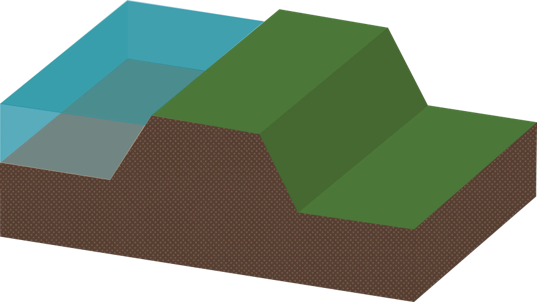
\includegraphics[width=0.75\linewidth]{figures/levee_graphic.png}
    \caption{General levee structure made from compacted earth.}
    \label{fig:levee}
\end{figure}

However, the database is known to be incomplete and contain incorrect coordinates for some levee paths, mostly due to a large portion of the early levee systems which were built by farmers and settlers up to centuries ago. An example of some of these inconsistencies can be found in \autoref{fig:missing}.

\begin{figure}[!h]
    \centering
    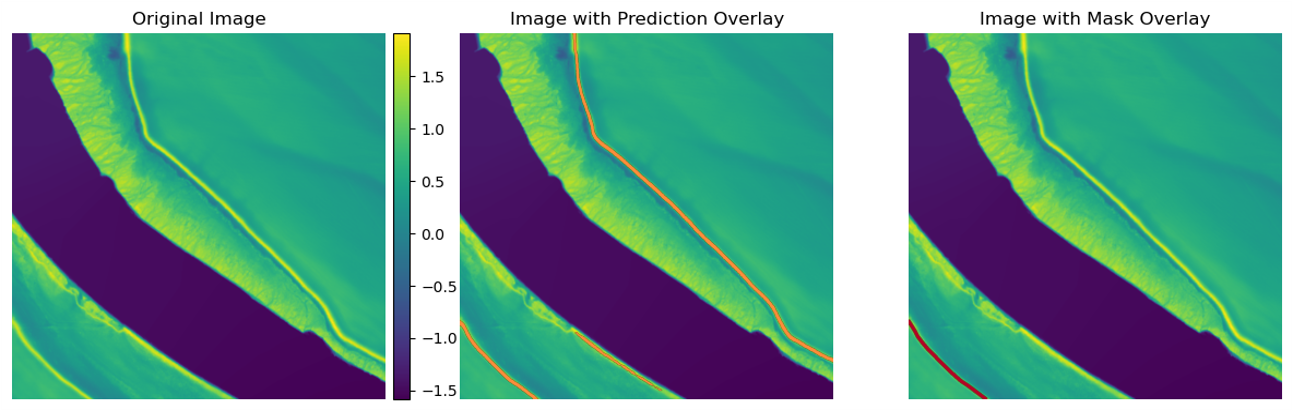
\includegraphics[width=0.75\linewidth]{figures/missing_levee.png}
    \caption{Missing levee in the database. "Image with prediction overlay" shows a missing levee which is not shown using the "mask overlay". This feature is also clearly seen in the original image with no overlays.}
    \label{fig:missing}
\end{figure}

These errors cause issues for Fathom, who need precise levee positions in order to produce highly accurate flood modelling data. These models are used across industries including humanitarian aid, insurance, international development, engineering, conservation, and financial markets.

We attempt to use the known levees to train a model for locating more levees from geospatial data, such as Light Detection and Ranging (LiDAR) data. This problem can be framed as a computer vision image segmentation task.

\section{Image Segmentation}
\label{sec:method}
%\input{method}
%---------------------------------------------------------------------

Image segmentation involves partitioning an image by assigning labels to individual pixels, effectively performing pixel-level classification. Unlike object detection, which uses boxes, or image classification, which assigns a single label to the entire image, segmentation identifies precise boundaries.

This technique is particularly valuable in fields like medicine - identifying organs, tumors, or blood vessels in CT and MRI scans - and autonomous driving - labelling roads, sidewalks, vehicles, and pedestrians.

For levee segmentation, LiDAR images are employed, where each pixel represents elevation instead of the typical three-channel (RGB) colour data.

The segmentation\_models.pytorch library provides a user-friendly API to several widely-used machine learning models for solving segmentation tasks efficiently. Within this project varieties of the UNet model \autoref{fig:unet}, and Segformer models were tested, with both providing equal results.

\begin{figure}[!h]
    \centering
    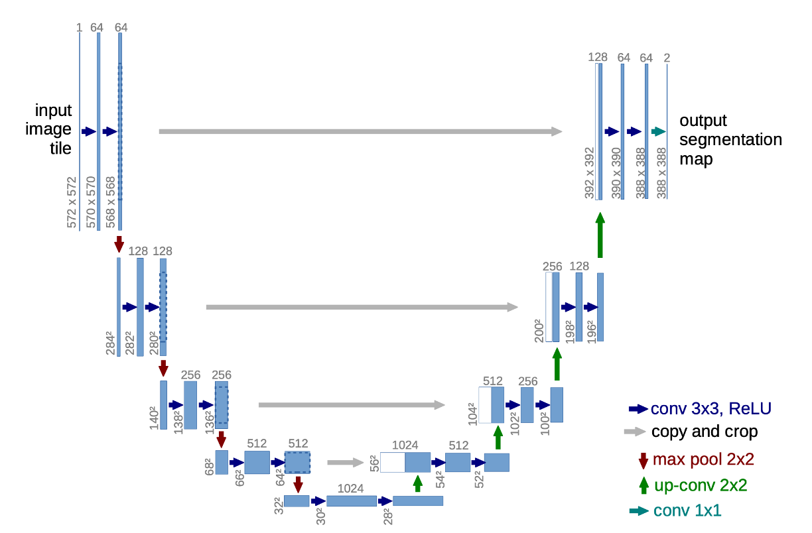
\includegraphics[width=0.75\linewidth]{figures/unet.png}
    \caption{UNet model architecture}
    \label{fig:unet}
\end{figure}

\section{Creating a pipeline}
\label{sec:results}
%\input{results}
%---------------------------------------------------------------------
\subsection{Data}

The data of known levees are downloaded from the NLD. Fathom provided a script, which uses the NLD2 API to query the database and downloads the levee data as gpkg format. The downloaded data contains about 7000 records, which are all the known levees in the US. These records only cover about a third of the existing levees in the U.S.A The levee data are used for creating masks as described in the next section.

Images of digital elevation models (DEMs) are used as the geospatial data for this project. DEM is a digital representations of the terrain elevation. They are usually derived from high-resolution LiDAR data, and levees can be identified as elevated features in the DEM images. This project uses the DEMs from the National Elevation Dataset (NED) distributed by the US Geological Survey (USGS). DEM images with different resolutions have been tested. The 1/3 arc-second resolution (roughly 10 meter) images can already reveal the existence of the levees and helps to build a working model. The one-meter resolution images give much better results, and would be the ideal choice if storage and computing resources allow. The DEM images are downloaded as GeoTIFF format via the TNM Access API provide by the National Map (TNM).

\subsection{Data Processing}

During model training, each image is paired with a corresponding mask - a binary image indicating the correct label for each pixel. In binary classification, target pixels (levees) are usually marked as 1, and background pixels as 0.

Masks are generated using an existing levee database, by matching geographical coordinates from LiDAR images with documented levee locations. The original images and their masks are then subdivided into smaller segments, ensuring dimensions remain divisible by 32, as required by segmentation models.

In the next step, all images containing invalid data are removed, and the number of images containing only background is limited.

Due to the incompleteness of the database, some masks contain inaccuracies. To mitigate this, images were manually reviewed, selecting or discarding those with unrealistic masks.

Ultimately, 49 areas near major U.S. cities with known levees were chosen to train the segmentation model.


\subsection{Model Training using K-Fold}

Standard K-Fold cross-validation divides the dataset into K part of equal size (folds); the model is then trained on K-1 folds of data, with testing on the remaining fold. This process is repeated K times, with each part being used once as the testing set. However, in real-world applications, data points aren't independent and can exist in defined groups, leading to over optimistic performance estimates as data from the same group exists in both the training and testing folds.

A "Group K-Fold Cross-Validation" method was used in this case to ensure that the smaller TIF images originating from each larger TIF image were split across groups (which are then evenly distributed to folds) and thus included in either the training set or the testing set for each fold. This helps prevent the model from learning and testing on an image from the same region (i.e. from the same original TIF file), improving model generalization to new, unseen data, while also providing realistic performance metrics, as future data will also be grouped the same way.

Following the GroupKFold, the model with the strongest metrics from the folds is selected to run inference, therefore, all the hyperparameters are saved in a JSON config file to be loaded in the inference pipeline.

The selected model is loaded using the saved hyperparameters and retrained using the full dataset, making use of the full dataset curated.
\subsection{Inference}

Inference is the final stage of the pipeline, where the full set of small TIF files from the USGS 3D Elevation Program can be input into the trained model to predict the presence of levees.

During inference, the images are passed through the segmentation model, outputting a probability mask indicating the likelihood of a levee's presence at each pixel. This probability mask then has a threshold applied and skeletonized to extract thin, continuous representations of the levees using a contour-based tracing algorithm. These vectorized line segments provide a clean and accurate geometric output. An example of this output can be found in \autoref{fig:13_arcsec_pred}, where 1/3~arcsec resolution data has been used for levee prediction using the UNet++ architecture.

\begin{figure}[!h]
    \centering
    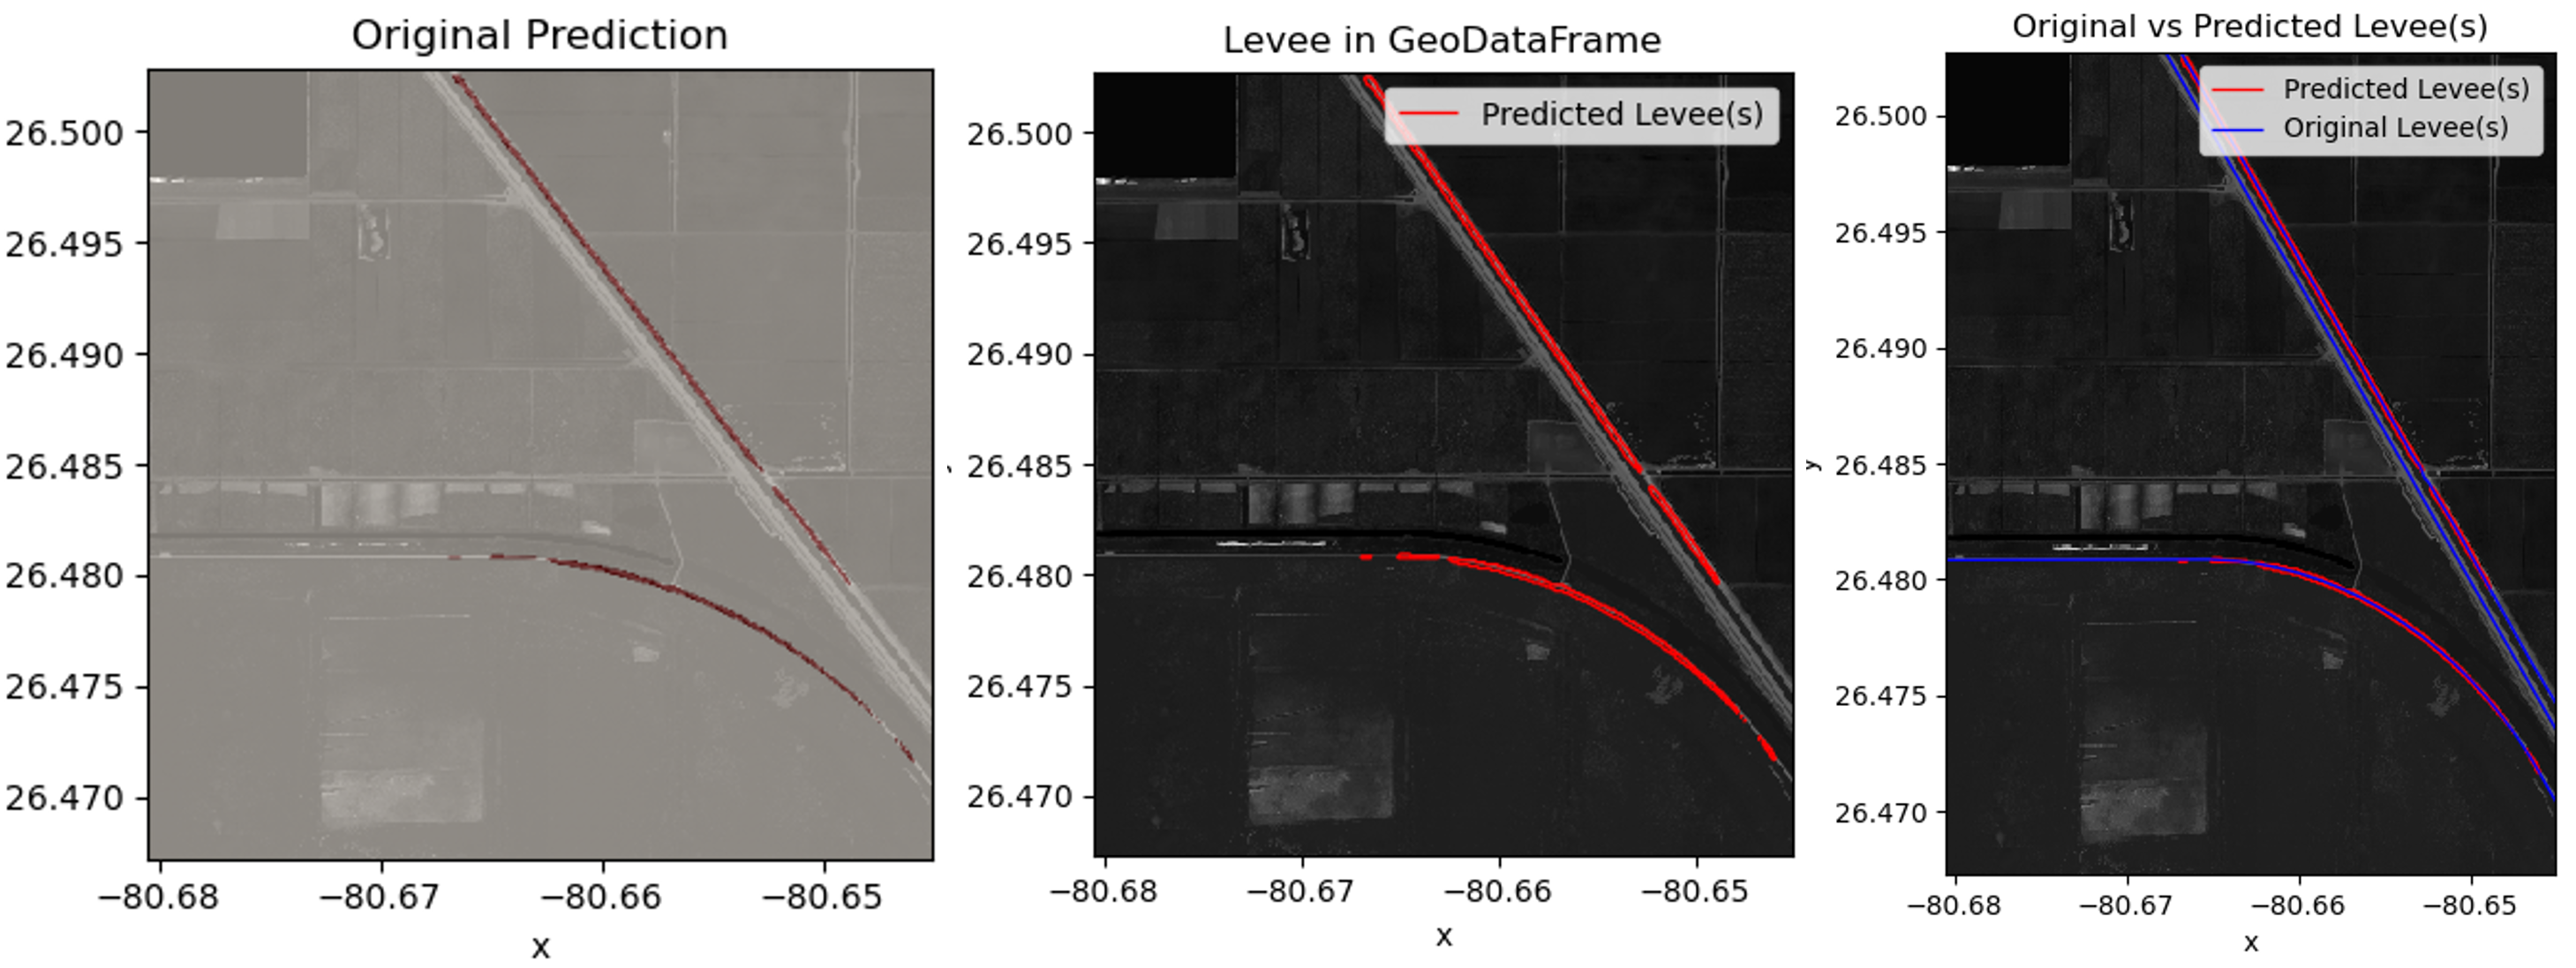
\includegraphics[width=0.75\linewidth]{figures/13_arcsec_performance.png}
    \caption{Levee prediction using 1/3 arcsec resolution DEM images overlayed with the original levees.}
    \label{fig:13_arcsec_pred}
\end{figure}

These line segments are assembled into a GeoPandas GeoDataFrame and saved in a GeoPackage, consistent with the original levees.gpkg file sourced from the National Levee Database (NLD). This ensures compatibility with existing geospatial workflows and allows for direct comparison between inferred and known levee locations.

\newpage
\section{Conclusions}
\label{sec:conclusion}
%\input{conclusion}
%---------------------------------------------------------------------
\begin{itemize}
    \item Image segmentation algorithms show good results for detecting levees using images from DEMs.
    \item This pipeline provides Fathom with the means to predict levees with the hope of finding new levees not in the NLD, while also potentially correcting any errors present.
    \item Further work to improve the models at 1/3~arcsec resolution is required, however a clear proof of concept is demonstrated.
    \item With no constraints on data storage, only minor adjustments to the pipeline would need be made to accommodate higher resolution images (1~m), greatly improving accuracy and performance.
    \item This project is open and publicly available, allowing anyone to follow the provided instructions and apply the approach to their own data and use cases.
\end{itemize}
%---------------------------------------------------------------------
\end{document}
